\documentclass[journal]{IEEEtran}

\usepackage[font=normalsize,labelfont=bf,hypcap=false]{caption}
\DeclareCaptionType{equ}[Eqn.][]
\usepackage{amsmath}
\usepackage{booktabs}
\usepackage[export]{adjustbox}
\usepackage{wrapfig}
\usepackage{optidef}
\usepackage[dvipsnames]{xcolor}
\usepackage[intoc, english]{nomencl}
\makenomenclature  %https://www.overleaf.com/learn/latex/Nomenclatures
\usepackage{lipsum}
\usepackage{tabularx}
\usepackage{color}
\usepackage{amsmath,amsfonts,amssymb,amscd}
\usepackage{graphicx}
\usepackage{epstopdf}
\usepackage{cite}
\usepackage{booktabs}
\usepackage{paralist}
\usepackage{multicol}
\usepackage{textcomp,gensymb}
\usepackage{steinmetz}
\usepackage{mathtools}
\usepackage{siunitx}
\usepackage{hyperref}
\usepackage{wrapfig}
\usepackage{svg}
\usepackage{mathrsfs}
\usepackage{comment}
\usepackage{color}
\usepackage{amsmath}
\usepackage{breqn}
\usepackage{colortbl}
\setlength\extrarowheight{1pt}
\usepackage[export]{adjustbox}
\usepackage{makecell}
\usepackage{multirow}
\usepackage{color}
\usepackage{float}

\usepackage{pifont}
\newcommand{\cmark}{\ding{51}}
\newcommand{\xmark}{\ding{55}}

% correct bad hyphenation here
\hyphenation{op-tical net-works semi-conduc-tor}


\begin{document}
\title{Influence of Loop Delay on \\LLC Converter Control Bandwidth}

\author{Nick~James~Kirkby,~\IEEEmembership{Student Member,~IEEE, njk@asu.edu}} % <-this % stops a space

\markboth{}
{Shell \MakeLowercase{\textit{et al.}}: Influence of Loop Delay on LLC Converter}


\maketitle

\begin{abstract}
A 1.5 MHz LLC converter is modeled analytically and in simulation to answer the question: what is the upper limit on stable control bandwidth given the sensing, computation, and actuation delays of the TMS320F28379D SOC?
\end{abstract}

\begin{IEEEkeywords}
LLC converter, delay modeling.
\end{IEEEkeywords}


\IEEEpeerreviewmaketitle


\section{Introduction}
\IEEEPARstart{P}{ower} converters such as the LLC are increasingly pushed to switching frequencies greater than 1 MHz to achieve miniaturization. 
At these high switching frequencies, delays due to sensing, control, and actuation may significantly reduce the closed-loop control bandwidth.
This paper investigates the influence of these delays on the control bandwidth of a 1.5 MHz LLC converter.

\section{System Model}

The system model is shown in Figure \ref{fig:feedback_diagram}. 
It consists of a plant $G_p(s)$, a controller $G_c(s)$, and a feedback delay $G_D(s)$.
The achievable control bandwidth may be limited by any of the three components in the feedback loop.
The aim of this project is to determine which of $ \{ G_c(s), G_p(s), G_D(s) \} $ limits the control bandwidth of the LLC converter implementation described in section \ref{sec:LLC_converter}.

\begin{figure}[H]
  \centering
  \includegraphics[width=0.5\textwidth]{figures/feedback_diagram.png}
  \caption{Feedback system model showing the plant $G_p(s)$, the controller $G_c(s)$, and the feedback delay $G_D(s)$.}
  \label{fig:feedback_diagram}
\end{figure}


\section{Plant Model}

Dynamic modeling of LLC converters is an active research area. 
The LLC converter is a nonlinear plant -- its dynamics vary as a function of both the control variable $f_s$ and also the load resistance $R_L$. 
The author selected Tian's plant transfer functions as derived in \cite{tian_equivalent_2020} as the basis for the plant model $G_p$. 

Tian's model has more than ten parameters. 
To check that the model was implemented correctly, the author compared the frequency response of the analytical plant model to the frequency response of a PLECS simulation of the same converter.

\subsection{Consistency between Analytical and Simulation Models}

Validation of the analytical model in simulation proved challenging as the LLC is frequency modulated and circuit simulation softwares vary greatly in their abilities to extract frequency response information from frequency-modulated switching converters.
An LLC converter was modeled in PLECS based on an example implemenation and multitone analysis \cite{plecs_analysis_2022} was used to extract its frequency response. 
The circuit is shown in Figure \ref{fig:PLECS_LLC}, where the small-signal perturbation is applied to the switching frequency $\omega_s$ and the output voltage $v_{o}$ is the response.

\begin{figure}
  \centering
  \includegraphics[width=0.5\textwidth]{figures/PLECS_LLC_schematic.png}
  \caption{LLC converter as modeled in PLECS and used to reproduce Tian's simuluation results.}
  \label{fig:PLECS_LLC}
\end{figure}

Initial comparison between simulated frequency response and the analytical transfer functions created using Tian's method did not agree. The comparison is shown in Figure \ref{fig:PLECS_Tian_comparison} where each model is evaluated using the converter parameters from Fig. 22 of \cite{tian_equivalent_2020}. The outputs agree closely for the $F_s = 1.4 F_o$ case, but disagree for the remaining two cases.

\begin{figure}
  \centering
  \includegraphics[width=0.5\textwidth]{figures/tian_vs_PLECS_disagreement.png}
  \caption{Comparison of simulated frequency responses of the same converter implemented in PLECS (dashed lines) and $G_p(s)$ using Tian's method (solid lines) at ${F_s=\{1.4, 1.0, 0.8\}F_o}$ using converter parameters from Fig. 22 of \cite{tian_equivalent_2020}. The discrepancy was found to stem from nonideal diode models used in the PLECS simulation.}
  \label{fig:PLECS_Tian_comparison}
\end{figure}

To gain confidence in the simulated frequency response results, the PLECS multitone analysis was compared alongside Tian's SIMPLIS implementation. 
The comparison is shown in Figure \ref{fig:simulation_comparison} where the PLECS and SIMPLIS frequency responses are nearly identical. 
PLECS' multitone and SIMPLIS' periodic operating point (POP) analysis methods differ in their implementations, but both are able to extract closely matching frequency responses of the modeled converter. 
The parameters in the PLECS simulation were updated to match those in the SIMPLIS simulation provided to the author by Dr. Tian.

\begin{figure}
  \centering
  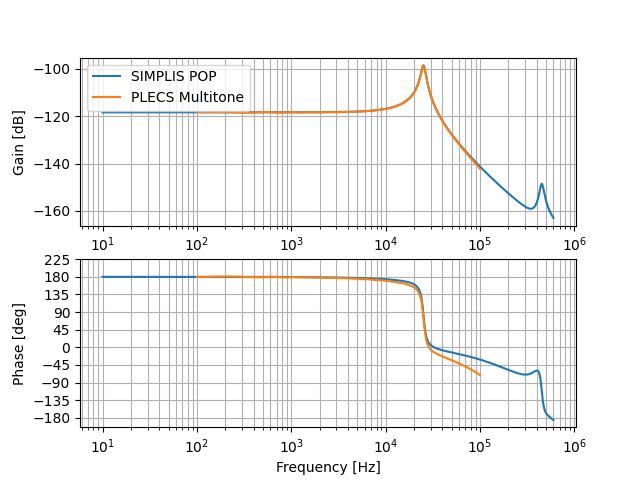
\includegraphics[width=0.5\textwidth]{figures/SIMPLIS_PLECS_comparison.png}
  \caption{Comparison of simulated frequency responses of the same converter implemented in PLECS and SIMPLIS circuit simulators. }
  \label{fig:simulation_comparison}
\end{figure}

The source of the discrepancy in Figure \ref{fig:PLECS_Tian_comparison} was traced back to nonideal diode models in the PLECS simulation which the author adapted from a PLECS example. 
The second-order resonant peak in visible in the ${F_s=1.0F_o}$ and ${F_s=0.8F_o}$ cases is very sensitive to rectifier damping, and the simulated diode losses in the PLECS example implementation were sufficient to fully damp the resonant peak predicted by the analytical model for an LLC converter with a lossless rectifier.
With the discrepancy understood, the 1.5 MHz LLC converter was modeled next.

\subsection{Modeling the 1.5 MHz LLC Converter}
\label{sec:LLC_converter}

The parameters in Table \ref{tab:llc_parameters} were used to model the 1.5 MHz LLC converter in the remainder of this paper. 
This converter is designed to deliver 1500 W at 48 V from a 270 V input.
The 1500 W operating point is at $F_s = 1.0 F_o$, so \cite{tian_equivalent_2020} Eqn. 14 ($F_s \ge F_o$) is used to model the plant. 
In this 1.5 MHz LLC converter, a full-bridge inverter is used instead of the half-bridge inverter used in \cite{tian_equivalent_2020}.
Due to the voltage-doubling effect of the full bridge inverter, the control-to-output plant transfer function $G_p(s) = \frac{v_o(s)}{\omega_s(s)}$ is a factor of two larger than the half-bridge case derived by Tian ~\cite{tian_equivalent_2020}, Eqn. 14. 
A schematic of the new 1.5 MHz LLC converter with full-bridge inverter is shown in Figure \ref{fig:PLECS_FB_LLC}.

\begin{table}[H]
\centering
\begin{tabular}{|c|c|c|c|}
\hline
\textbf{Parameter} & \textbf{Value}  & \textbf{Description} \\ \hline
$L_r$ & 2 $\mu H$ & Resonant inductor \\ \hline
$L_m$ & 10 $\mu H$ & Magnetizing inductor \\ \hline
$C_r$ & 5.6 $nF$ & Resonant capacitor \\ \hline
$C_f$ & 100 $\mu F$ & Output filter capacitor \\ \hline
$n_{pri}$ & 6 & Transformer primary turns \\ \hline
$n_{sec}$ & 1 & Transformer secondary turns \\ \hline
$R_{load}$ & 1.536 $\Omega$ & Load resistance \\ \hline
$V_{o}$ & 48 $V$ & Output voltage \\ \hline
$V_{g}$ & 270 $V$ & Input voltage \\ \hline
$P_{o}$ & 1500 $W$ & Output power \\ \hline
$F_{o} = \frac{1}{2\pi\sqrt(L_r C_r)}$ & 1.5 $MHz$ & Resonant tank frequency \\ \hline
\end{tabular}
\caption{LLC converter parameters used in the remainder of this paper.}
\label{tab:llc_parameters}
\end{table}

\begin{figure}
  \centering
  \includegraphics[width=0.5\textwidth]{figures/PLECS_FB_LLC_schematic.png}
  \caption{LLC converter with full-bridge inverter.}
  \label{fig:PLECS_FB_LLC}
\end{figure}

Finally, the analytical and simulated models were compared for the 1.5 MHz LLC using the parameters shown in Table \ref{tab:llc_parameters}, and the resulting frequency responses are compared in Figure \ref{fig:MHZ_open_loop_plant_PLECS_validation}. 
The agreement of the two models is excellent, and the analytical plant model is used for compensator design in the following section.

\begin{figure}
  \includegraphics[width=0.5\textwidth]{figures/MHz_open_loop_plant_PLECS_validation.png}
  \caption{Cross-validation of plant frequency responses of $G_p(s)$ based on \cite{tian_equivalent_2020} and PLECS simulation for a full-bridge LLC converter using the parameters given in Table \ref{tab:llc_parameters}.}
  \label{fig:MHZ_open_loop_plant_PLECS_validation}
\end{figure}

\section{Compensator Design}
\label{sec:compensator_design}

The open-loop plant transfer function corresponding to the LLC converter with parameters in Table \ref{tab:llc_parameters} is shown in Fig. \ref{fig:MHZ_open_loop_plant_PLECS_validation} and as a transfer function in (\ref{eq:open_loop_plant}).

\begin{equ}[h]
\begin{equation}
G_p = 
\frac{v_o(s)}{\omega_s(s)} = \frac{-1.401 \times 10^{12}}{9.959 \times 10^{6} s^2 + 7.23 \times 10^{10} s + 7.2 \times 10^{17}}
\label{eq:open_loop_plant}
\end{equation}
\end{equ}

The plant transfer function (\ref{eq:open_loop_plant}) contains a pole pair at the resonant frequency of the output capacitance and the effective tank inductance. 


The controller $G_c$ was designed using the k-factor method \cite{venable_k_1983} as taught by Dr. Raja Ayannar \cite{ayannar_k-factor_2014,ayannar_k_2014}, with some minor modifications. The controller design steps are as follows:

\begin{enumerate}
  \item Determine the phase of the plant, $\phi_{sys}$ at $\omega_c$ from analytical small signal model (\ref{eq:open_loop_plant}).
  \item Calculate phase boost $\phi_{boost}$ required, using $\phi_{boost} = PM_{desired} - \phi_{sys} - 90\degree$.
  \item Calculate $k$, $\omega_z$, and $\omega_p$ as follows: $k = tan(\frac{\phi_{boost}}{2})$, $\omega_z = \frac{\omega_c}{k}$, and $\omega_p = k \omega_c$.
  \item Calculate $K_c$, $K_c = \frac{\omega_c}{k|G_p(j\omega_c)|}$.
\end{enumerate}

The sign of the plant transfer function $G_p$ is negative, so $180\degree$ was added to $\phi_{sys}$ to compensate for its negative sign.
The form of the type-II k-factor controller is

\begin{equ}[h]
\begin{equation}
  G_c = \frac{K_c}{s} \frac{1 + \frac{s}{\omega_z}}{1 + \frac{s}{\omega_p}}
\label{eq:type_II_k_factor}
\end{equation}
\end{equ}

The forward-path transfer function $G_c G_p$ is the product of (\ref{eq:type_II_k_factor}) and (\ref{eq:open_loop_plant}).

The phase margin $PM_{desired}$ and the crossover frequency $\omega_c$ were swept over the ranges $\{ 60,90 \} \degree$ 
and $\{ 300,5000 \} Hz$ respectively and the closed loop step response and gain margin were observed. 
Fig. \ref{fig:oltf} shows the open-loop transfer function $G_c G_p$ for a type-II k-factor controller with $PM_{desired} = 85\degree$ and $f_c = 1000$ Hz.
The gain margin is more than 6 dB with the crossover frequency at 1000 Hz.
Further increasing the crossover frequency reduces the gain margin unacceptably.

\begin{figure}
  \includegraphics[width=0.5\textwidth]{figures/85deg_PM_at_1000_Hz_OLTF.png}
  \caption{$G_c G_p$ where $G_c$ is a type-II k-factor controller with $PM_{desired} = 85\degree$ and $f_c = 1000$ Hz.}
  \label{fig:oltf}
\end{figure}

The step response of three controller variants is shown in Fig. \ref{fig:step_response_for_different_fc}.
The instability due to decreasing gain margin is visible in the third case $f_c = 5000$ Hz.
The best closed loop response was found at $PM_{desired} = 85\degree$ and $f_c = 1000$ Hz, $(\omega_c = 6283 \frac{rad}{s})$.

\begin{figure}
  \includegraphics[width=0.5\textwidth]{figures/step_response_for_different_fc.png}
  \caption{Closed-loop step response for three crossover frequency values $f_c$.}
  \label{fig:step_response_for_different_fc}
\end{figure}

Finally, the closed-loop frequency responses of the analytical model and the PLECS simulation were compared. 
The results are shown in Figure \ref{fig:closed_loop_freq_response}.

\begin{figure}
  \includegraphics[width=0.5\textwidth]{figures/closed_loop_comparison.png}
  \caption{Comparison of $G_{cl} = \frac{G_c G_p}{1 + G_c G_p}$ for the analytical model (solid line) and PLECS simulation (dashed line).}
  \label{fig:closed_loop_freq_response}
\end{figure}

\section{Delay Modeling}

The original aim of this project was to find which of $\{ G_c(s), G_p(s), G_D(s) \} $ limits the control bandwidth of the LLC converter.
Section \ref{sec:compensator_design} showed that the plant $G_p(s)$ limits the control bandwidth to approximately 1 kHz due to the lightly-damped plant double pole at approximately 40 kHz.
As the controller bandwidth is increased beyond 1 kHz, proximity to the double plant pole at 40 kHz results in a diminishing gain margin and closed-loop stability is compromised.

Practically speaking, a 1 kHz bandwidth controller is trivial to implement on the TMS320F28379D SOC, and further analysis of $G_D$ is not necessary.
However, the author has included a brief analysis of the delay model for completeness.
Also, an alternate 1.5 MHz LLC design in which the size of the filter capacitor $C_f$ is decreased in order to push the 40 kHz plant double pole to a higher frequency is of interest to the author.
A sufficient decrease in filter capacitance $C_f$ will eventually result in the control bandwidth being limited by controller delays $G_D$ instead of plant dynamics $G_p$.

\subsection{Analytical Delay Model}

Using chapter 6.8 of \cite{franklin_feedback_2019}, the effects of time delays in the controller are modeled using a Pade approximation (\ref{eq:delay_approximation}).

\begin{equ}[h]
\begin{equation}
    \angle G_D = -\omega T_d 
\label{eq:delay_approximation}
\end{equation}
\end{equ}

where $T_d$ is the delay time, $\omega$ is the frequency in $\frac{rad}{s}$, and $\angle G_D$ is the phase delay in $rad$.

For an embedded control application, sensing, computation and actuation are designed to run at a fixed frequency with deterministic execution time.
Fig. \ref{fig:pade_delay_for_different_loop_frequencies} shows the phase delay contributed for four candidate loop periods of $T = \{1, 2, 10, 20\} \mu s$.
A phase delay of more than $10\degree$ is considered undesirable.
It can be seen from Figure \ref{fig:pade_delay_for_different_loop_frequencies} that even the slowest considered loop period of 20 $\mu s$ does not contribute significant phase delay 1 kHz.

\begin{figure}
  \includegraphics[width=0.5\textwidth]{figures/pade_delay_for_different_loop_frequencies.png}
  \caption{Approximation of delay angle contribution $\angle G_d$ versus frequency for four loop frequencies calculated using (\ref{eq:delay_approximation}).}
  \label{fig:pade_delay_for_different_loop_frequencies}
\end{figure}

For control bandwidths exceeding 10 kHz, the phase delay contribution will become significant. This is the subject of future analysis.

\section{Conclusion}

The analytical transfer functions of the LLC converter provided in \cite{tian_equivalent_2020} were validated against a PLECS simulation.
A 1.5 MHz LLC was modeled and its plant transfer function used to design a type-II k-factor controller.
It was found that the control bandwidth is limited by the plant double pole at approximately 40 kHz, and that delays due to sensing, computation, and actuation do not limit the control bandwidth of the 1.5 MHz LLC converter studied here.

% if have a single appendix:
%\appendix[Proof of the Zonklar Equations]
% or
%\appendix  % for no appendix heading
% do not use \section anymore after \appendix, only \section*
% is possibly needed

% use appendices with more than one appendix
% then use \section to start each appendix
% you must declare a \section before using any
% \subsection or using \label (\appendices by itself
% starts a section numbered zero.)
%




% use section* for acknowledgment
\section*{Acknowledgments}

Dr. Shuilin Tian provided crucial support in reproducing his results. 
Dr. Jennie Si gave valuable feedback and guidance during this project.

% Can use something like this to put references on a page
% by themselves when using endfloat and the captionsoff option.
\ifCLASSOPTIONcaptionsoff
  \newpage
\fi



% trigger a \newpage just before the given reference
% number - used to balance the columns on the last page
% adjust value as needed - may need to be readjusted if
% the document is modified later
%\IEEEtriggeratref{8}
% The "triggered" command can be changed if desired:
%\IEEEtriggercmd{\enlargethispage{-5in}}

% references section

% can use a bibliography generated by BibTeX as a .bbl file
% BibTeX documentation can be easily obtained at:
% http://mirror.ctan.org/biblio/bibtex/contrib/doc/
% The IEEEtran BibTeX style support page is at:
% http://www.michaelshell.org/tex/ieeetran/bibtex/
%\bibliographystyle{IEEEtran}
% argument is your BibTeX string definitions and bibliography database(s)
%\bibliography{IEEEabrv,../bib/paper}
%
% <OR> manually copy in the resultant .bbl file
% set second argument of \begin to the number of references
% (used to reserve space for the reference number labels box)
% \begin{thebibliography}{1}

% \bibitem{IEEEhowto:kopka}
% H.~Kopka and P.~W. Daly, \emph{A Guide to \LaTeX}, 3rd~ed.\hskip 1em plus
%   0.5em minus 0.4em\relax Harlow, England: Addison-Wesley, 1999.

% \end{thebibliography}

{\vspace{\baselineskip}
	\bibliographystyle{IEEEtran}
	\bibliography{bibliography}
}

% biography section
% 
% If you have an EPS/PDF photo (graphicx package needed) extra braces are
% needed around the contents of the optional argument to biography to prevent
% the LaTeX parser from getting confused when it sees the complicated
% \includegraphics command within an optional argument. (You could create
% your own custom macro containing the \includegraphics command to make things
% simpler here.)
%\begin{IEEEbiography}[{\includegraphics[width=1in,height=1.25in,clip,keepaspectratio]{mshell}}]{Michael Shell}
% or if you just want to reserve a space for a photo:

% \begin{IEEEbiography}{Michael Shell}
% Biography text here.
% \end{IEEEbiography}

% % if you will not have a photo at all:
% \begin{IEEEbiographynophoto}{John Doe}
% Biography text here.
% \end{IEEEbiographynophoto}

% % insert where needed to balance the two columns on the last page with
% % biographies
% %\newpage

% \begin{IEEEbiographynophoto}{Jane Doe}
% Biography text here.
% \end{IEEEbiographynophoto}

% You can push biographies down or up by placing
% a \vfill before or after them. The appropriate
% use of \vfill depends on what kind of text is
% on the last page and whether or not the columns
% are being equalized.

%\vfill

% Can be used to pull up biographies so that the bottom of the last one
% is flush with the other column.
%\enlargethispage{-5in}



% that's all folks
\end{document}


